\documentclass[addtable,twoside,12pt]{hynuexam2024}

%%%%%%%%%%%%%%%%使用XeLaTeX运行%%%%%%%%%%%%%%%%
%%%%%%%%%%%%%%%%使用XeLaTeX运行%%%%%%%%%%%%%%%%
%%%%%%%%%%%%%%%%使用XeLaTeX运行%%%%%%%%%%%%%%%%
%\printanswers				%%%%%%%%%%%显示答案就取消这个注释


%\usepackage{showframe}
%\usepackage{arev}
\usepackage{fouriernc}		 %%%数学公式字体宏包
\linespread{1.2}			 %%%行间距
\begin{document}

	%需要答案把\printanswers这个命令取消注释\documentclass[addtable,twoside,14pt]{hnuexam}
	%线性代数第一次平时作业——线性方程组的解，矩阵乘法与逆矩阵
	%%%%%%%%%%%%%%%%使用XeLaTeX运行%%%%%%%%%%%%%%%%
	%%%%%%%%%%%%%%%%使用XeLaTeX运行%%%%%%%%%%%%%%%%
	%%%%%%%%%%%%%%%%使用XeLaTeX运行%%%%%%%%%%%%%%%%
	%需要答案把\printanswers这个命令取消注释
	%需要答案把\printanswers这个命令取消注释
	%需要答案把\printanswers这个命令取消注释

	% 输出左边学生需要填写信息的表格
	%%%%%%%%%%%%%%%%%%%%%%%%%%%%%%%%% 学生考前需要填写的信息输出
	\examinformation%
	{衡阳师范学院\underline{2046-2047}学年\;第\underline{二}学期}%
	{高考数学全国卷$\left(\mathrm{\Rmnum{1}}\right)$\quad 期末考试试题\,A\,卷}%
	{（适用于\underline{2045}级\underline{数学与应用数学}专业本科学生）}%
	{闭卷}%
	{120}%

	\vspace{-1em}
	\sectiongradetable
	\vspace*{-0.5em}
	%%%%%%%%%%%%%%%%%%%%%%%%%%%%%%%%%%%%%%%%%%%%%%%%%%%%%%%%%%%%%%%%%%%%%%%%%%%%%%
	%可以在这里用下面这个命令写一些试卷的说明
	%%%%%%%%%%%%%%%%%%%%%%%%%%%%%%%%%%%%%%%%%%%%%%%%%%%%%%%%%%%%%%%%%%%%%%%%%%%%%%%
	%\centerline{\textbf{（注意：本试卷中的坐标架在没标明的情况下指的都是直角坐标架）}}

	\begin{questions}
		%\setcounter{question}{0}
		\makepart{简答题}[5]{10}
		\begin{EnvFullwidth}
			\setlength{\parindent}{2em} 请解以下的三角形问题以及圆锥曲面问题：
		\end{EnvFullwidth}
		\question 设$\triangle A B C$的内角$A, B, C$的对边分别为$a, b, C$, 已知$\sin C=\sqrt{2} \cos B$,
		$a^{2}+b^{2}-c^{2}=\sqrt{2} a b$
		\begin{enumerate}[(i)]
			\item 求$B$
			\item 若$\triangle A B C$的面积为$3+\sqrt{3}$, 求$C$
		\end{enumerate}
		\vspace*{\stretch{0.7}}

		\question 已知$A(0,3)$和$P\left(3, \dfrac{3}{2}\right)$为椭圆$ C: \dfrac{x^{2}}{a^{2}}+\dfrac{y^{2}}{b^{2}}=1(a>b>0)$上两点.
		\begin{enumerate}[(I)]
			\item 求$C$的离心率
			\item 若过P的直线$L$交$C$于另一点$B$, 且$\triangle A B P$的面积为9, 求$L$的方程
		\end{enumerate}
		\vspace*{\stretch{1}}
		\begin{solution}
			\begin{enumerate}[(1)]
				\item $\frac{1}{2}+\frac{1}{3}+\frac{1}{4}+\cdots+\cdot=\sum\limits_{n=1}^{\infty}\frac{1}{n+1}$\score{4}
				\item 先求前$n$项的和\begin{align*}
					S_n&=\frac{1}{1\cdot 2}+\frac{1}{2\cdot 3}+\frac{1}{3\cdot 4}+\cdots+\frac{1}{n(n+1)}\score{1}\\
					&=1-\frac{1}{2}+\frac{1}{2}-\frac{1}{3}+\frac{1}{3}-\frac{1}{4}+\cdots+\frac{1}{n}-\frac{1}{n+1}\score{3}\\
					&=1-\frac{1}{n+1}\score{4}\\
					\lim_{n\to\infty}S_n&=\lim_{n\to\infty}\left(1-\frac{1}{n+1}\right)=1\score{5}
				\end{align*}
				于是$\frac{1}{1\cdot 2}+\frac{1}{2\cdot 3}+\frac{1}{3\cdot 4}+\cdots+\frac{1}{n(n+1)}+\cdots=1$\score{6}
			\end{enumerate}
		\end{solution}
		\clearpage
		%\vspace*{\stretch{5}}

		\makepart{选择题}[2]{10}
		\question 已知集合$A=\left\{x \mid-5<x^{3}<5\right\}$, $B=\{-3,-1,0,2,3\} $, 则  $A \cap B$=\chABCD[]

		\begin{oneparchoices}
			\choice $\{-1,0\}$
			\choice $\{2,3\}$
			\choice $\{-3,-1,0\}$
			\choice $ \{-1,0,2\}  $
		\end{oneparchoices}

		\question  若$\dfrac{2}{z-1}=1+i$, 则$z=$\chABCD[]

		\begin{oneparchoices}
			\choice $1-i$
			\choice $-1+i$
			\choice $1-i$
			\choice $1+i $
		\end{oneparchoices}

		\question  已知向量$\vec{a}=(0,1) \cdot \vec{b}=(2,x)$, 若$\vec{b} \perp(\vec{b}-4\vec{a})$则$x=$\chABCD[]

		\begin{oneparchoices}
			\choice $-2$
			\choice  $-1$
			\choice  $1$
			\choice $2$
		\end{oneparchoices}

		\question  已知  $\cos (\alpha +\beta)=m$, $\tan \alpha  \tan \beta=2$, 则$\cos (\alpha -\beta)=$\chABCD[]

		\begin{oneparchoices}
			\choice $-3m$
			\choice $-\dfrac{m}{3}$
			\choice $\dfrac{m}{3}$
			\CorrectChoice  $3m$
		\end{oneparchoices}

		\question  已知圆柱和圆锥的底面半径相等, 侧面积相等, 且它们的高均为$\sqrt{3}$, 则圆锥的体积为\chABCD[]

		\begin{oneparchoices}
			\choice$2 \sqrt{3} \pi$
			\choice$3 \sqrt{3} \pi$
			\choice  $6 \sqrt{3} \pi$
			\CorrectChoice $9 \sqrt{3} \pi$
		\end{oneparchoices}

		\makepart{填空题}[2]{10}\setlength\fillinlinelength{1in}% 设置默认长度为1in
		\question 设双曲线$C: \dfrac{x^{2}}{a^{2}}-\dfrac{y^{2}}{b^{2}}=1(a>0, b>0)$的左右焦点分别为$F_{1}, F_{2}$, 过$ F_{2}$作平行于y轴的直成交C于$A, B$两点, 若$|FA|=13$, $|A B|=10$, 则的离心率为\fillanswer

		\question 若曲线$y=e^{x}+x$在点$(0.1)$处的切线也是曲线$ y=\ln (x+1)+a $的切线, 则$a=$\fillin

		\question 甲, 乙两人各有四张卡片, 每张卡片上椋有一个数字, 甲的卡片上分别标有数字1, 3, 5, 7, 乙的卡片上分别标有数字2, 4, 6, 8两人进行四轮比赛, 在每轮比赛中, 两人各自从自己持有的卡片中随机抽出一张, 并比较所选卡片上数字的大小, 数字大的人得分, 数字小的人得0分. 然后各自弃置此轮所达的卡片(弃置的卡牌在此后的轮次中不能使用). 则四轮比赛后, 甲的总得分不小于2的概率为\fillin[][2in]
		%%%%%%%%%%%%%%%%%%%%这里给出一个每个大题分数不一样的例子%%%%%%%%%%%%%%%%%%
		%% 请注意，这里\makepart命令只有两个参数，可选参数没有，因为有一些大题的分数不一样。
		\question 设 $S_n$ 为等差数列 $\left\{a_n\right\}$ 的前 $n$ 项和,  若 $a_3+a_4=7 $,    $3 a_2+a_5=5$ ,  则 $S_{10}=$ \fillin

		\question 已知 $\alpha,\beta$ 均为第一象限角,  $\tan \alpha+\tan \beta=4$ ,   $\tan \alpha \tan \beta=\sqrt{2}+1$ ,  则$\sin (\alpha+\beta)=$ \fillin

		\makepart{判断题}[2]{10}
		\question \torf[\CheckmarkBold]复数的模长$|-1-i|=\sqrt{2}$

		\question \torf[\XSolidBrush]已知命题: $p: \forall x \in \mathbb{R},    |x+1|>1$ ,    命题 $q: \exists x>0 $,     $x^3=x$ ,     则  $p$ 和 $q$ 都是真命题.

		\question \torf[\CheckmarkBold]已知向量 $\vec{a}$ ,     $\vec{b}$ 满足 $|\vec{a}|=1 $,     $|\vec{a}+2 \vec{b}|=2$ ,    且 $(\vec{b}-2 \vec{a}) \perp \vec{b}$ ,    则 $|\vec{b}|=\frac{\sqrt{3}}{2}$

		\question \torf[\XSolidBrush]已知曲线 $C: x^2+y^2=16 ~(y>0)$,    从 $C$ 上任意一点 $P$ 向 $x$ 轴作垂线段 $P P^{\prime},    P^{\prime}$为垂足,    则线段 $P P^{\prime}$ 的中点 $M$ 的轨迹方程为 $\frac{x^2}{16}+\frac{y^2}{4}=1 ~(y>0)$

		\question \torf[\CheckmarkBold]对于函数 $f(x)=\sin 2 x$ 和 $g(x)=\sin \left(2 x-\frac{\pi}{4}\right)$,
		$f(x)$ 与 $g(x)$ 的图像有相同对称轴
		%不定积分$\displaystyle\int e^{x^2}\,\mathrm{d}x=e^{x^2}+C$

		\clearpage

		\makepart{解答题}[10]{50}
		\question 已知函数 $f(x)=e^x- x-1$. 求曲线 $y=f(x)$ 在点 $(1,   f(1))$ 处的切线方程；
		\begin{solution}%%%%%%%%%%%%%%%%%%%%%%%%这是解答过程
			解：这是解答过程\score{2}
			\begin{align*}
				y&=x^2+x-x+1\score{8}\\
				&=x^2+1\score{10}
			\end{align*}
		\end{solution}
		%%%%%%%%%%%%%%%%%%%%%%%%%%%%%%%%%%%%%%%%%%%%%%%%%%%%%%%%%%%%%%%%%%%%%%%%%%%%%%%%%%%%%%%%%
		%\vspace*{\stretch{1}}
		%使得这个命令留出作答的空白，如果要留宽一点把这个数字设置得更大一点即可
		%%%%%%%%%%%%%%%%%%%%%%%%%%%%%%%%%%%%%%%%%%%%%%%%%%%%%%%%%%%%%%%%%%%%%%%%%%%%
		\vspace*{\stretch{0.8}}


		%\clearpage%%%%%%%%%%%%%%%%%%%%%%%%%%%%%%%%%%%%%%%%%%%%%%%%%%%%%%%%%%%%%%%%%%%%%%%%%%%%%使用该命令强制换页
		\question 设函数 $f(x)=(x+a) \ln (x+b)$,   若 $f(x) \geqslant 0$,   试求 $a^2+b^2$ 的最小值.

		\vspace*{\stretch{1.2}}

		\question 如图, 四棱锥$P-ABCD$中, $PA\perp$地面$ABCD$, $PA=AC=2$, $PBC=1$, $AB=\sqrt{3}$
		\begin{enumerate}[(a)]
			\item 若$AD \perp PB$, 记明: $AD\parallel$ 平面 $PBC$
			\item 若$AD\perp DC$, 且二面用$A-CP-D$的政弦值为$\dfrac{\sqrt{42}}{7}$, 求$AD $
		\end{enumerate}
		\begin{flushright}
			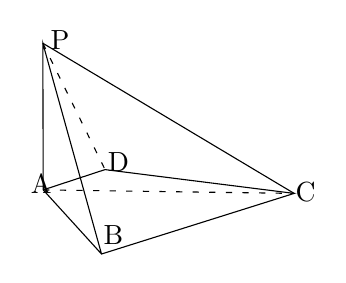
\begin{tikzpicture}[x=0.75pt,y=0.75pt,yscale=-1,xscale=1]
				%uncomment if require: \path (0,300); %set diagram left start at 0, and has height of 300

				%Straight Lines [id:da07947286263339692]
				\draw    (168.2,180.56) -- (139.92,79) -- (140.11,149.67) -- (168.2,180.56) -- (261,151.36) -- (169.89,139.89) -- (140.11,149.67) ;
				%Straight Lines [id:da2512301015844689]
				\draw    (139.92,79) -- (261,151.36) ;
				%Straight Lines [id:da7430017137368916]
				\draw  [dash pattern={on 2.25pt off 3.75pt on 2.25pt off 3.75pt}]  (139.92,79) -- (169.89,139.89) ;
				%Straight Lines [id:da9727208172737682]
				\draw  [dash pattern={on 2.25pt off 3.75pt on 2.25pt off 3.75pt}]  (140.11,149.67) -- (261,151.36) ;

				% Text Node
				\draw (138,71.78) node [anchor=north west][inner sep=0.75pt]   [align=left] {{ P}};
				% Text Node
				\draw (132.89,140.89) node [anchor=north west][inner sep=0.75pt]   [align=left] {{A}};
				% Text Node
				\draw (168,165.56) node [anchor=north west][inner sep=0.75pt]   [align=left] {{B}};
				% Text Node
				\draw (260.44,145.11) node [anchor=north west][inner sep=0.75pt]   [align=left] {{C}};
				% Text Node
				\draw (170,130.33) node [anchor=north west][inner sep=0.75pt]   [align=left] {{D}};
			\end{tikzpicture}
		\end{flushright}
		\vspace*{\stretch{1}}


		\clearpage
		\question 记 $\triangle A B C$ 的内角 $A$ 、 $B$ 、 $C$ 的对边分别为 $a$ 、 $b$ 、 $c$,   已知 $\sin A+\sqrt{3} \cos A=2$. 求 $A$.
		\vspace*{\stretch{1}}

		\question 已知函数$f(x)=\ln \dfrac{x}{2 x}+a x+b(x-1)^{3}$
		\begin{enumerate}[(1)]
			\item 若$b=0 $, 且$f^{\prime}(x) \geqslant 0$, 求$a$的最小值
			\item 证明: 曲线$y=f(x) $是中心对称图形
			\item 若$f(x)>-2$当且仅当$1<x<2$, 求$b$的取值范用。
		\end{enumerate}
		\vspace*{\stretch{1}}

		\makepart{证明题}[10]{10}
		\question 设$m$为正整数, 数列$a_{1}$, $ a_{2}$, $\cdots$ $a_{4 m+2}$是公差不为$ 0 $的等差数列, 若从中删去两项$a_{i}$和$a_{j}(i<j)$后剩余的$4m$项可被均分为m组, 且每组的4个数都能构成等差数列, 则称数列$a_{1}, a_{2}, \cdots, a_{4m+2}$是$(i, j  )$一可分数列
		\begin{enumerate}[(A)]
			\item 写出所有的$( i, j)$,   $1 \leq i j \leq 6$ , 使数到$a_{1}, a_{2}, \cdots, a_{6} $是$(i, j)$—可分数列.
			\item 当$m  \geqslant 3$时, 证明: 数列$ a_{1}, a_{2}, \cdots, a_{4m+2}$是$(2,13)$一可分数列
		\end{enumerate}
		\vspace*{\stretch{1}}
	\end{questions}
\end{document}